%!TEX root = ./Thesis.tex
\chapter{Discrete Differential Geometry - Software Packages}

In the field of Discrete Differential Geometry (DDG) there is a special need for experiments
conducted with the help of computer software. Especially if the methods of DDG are applied
to problems in computer graphics, geometry processing, or architecture, algorithms have 
to be implemented and convincing examples have to be presented. Additionally a suitable 
visualization of the results has to be included in a state-of-the-art publication.

There is a growing knowledge of software development in the mathematical community. This 
is partly due to the curricula of universities which started to include programming courses for undergraduate students.
This enables the students to extend their abilities of creating visualizations and mathematical software, where former generations of students solely used Mathematica and MatLab.

This Chapter is the description and getting-started manual of a set of software packages
(DDG Framework) written in Java. They are specifically designed for the creation of custom interactive software
for experiments with algorithms and geometries treated within DDG. 
Section~\ref{sec:jrworkspace} introduces the {\sc JRWorkspace} library of the {\sc Jtem} project~\cite{JtemWebsite}.
It is the foundation of any application created with the DDG Framework. It is also the user interface basis of {\sc Jreality}, a mathematical visualization library that uses {\sc JRWorkspace} as plug-in and user interface tool~\cite{JrealityWebsite}. In Section~\ref{sec:conformallab} we describe the software {\sc ConformalLab}. This package
implements the methods of the publications~\cite{Bobenko2010, OWR2012, Sechelmann2012, BobSechSpr}.
Section~\ref{sec:varylab} introduces {\sc VaryLab} the software implementation of the methods described in the publications \cite{Lafuente2011, Lafuente2012, Sechelmann2012}.
This package is also released to partners of the development group as {\sc VaryLab[Gridshells]}, {\sc VaryLab[Ultimate]}, or even online as {\sc VaryLab[Service]}.

\begin{figure}
	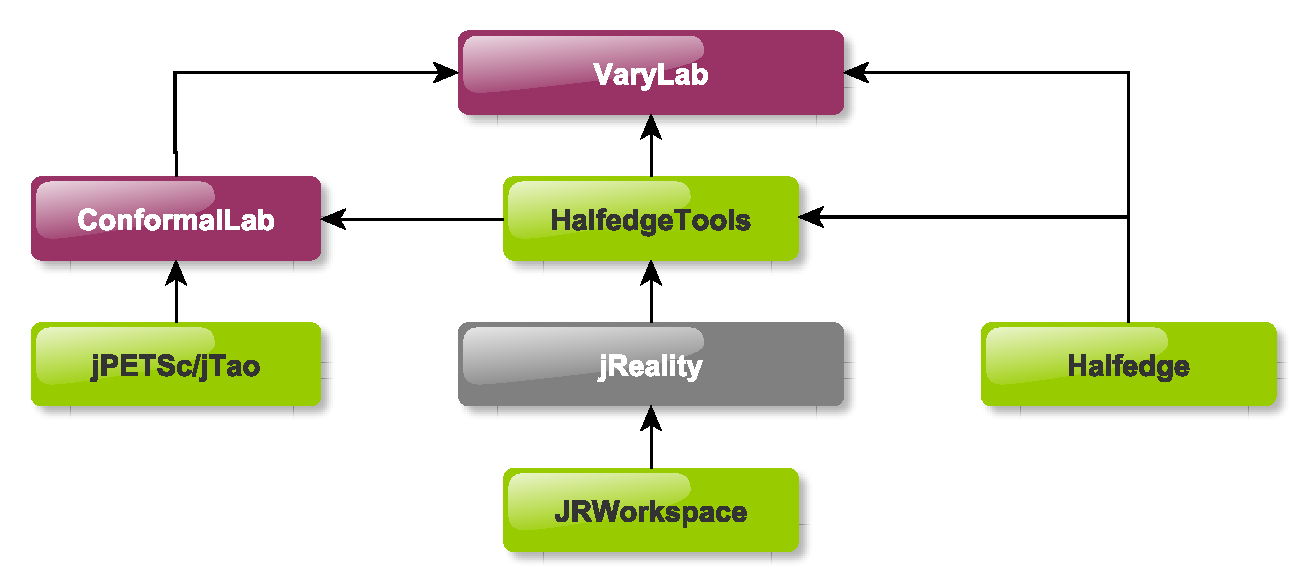
\includegraphics[width=\linewidth]{figures/software_architecture}
	\caption{Software architecture of the DDG Framework}
	\label{fig:software_architecture}
\end{figure}

\section{{\sc JRWorkspace} - A plug-in driven GUI library}

\label{sec:jrworkspace}
\subsection{Plug-ins}
\subsection{Gui elements}
\subsection{{\sc JRWorkspace} and {\sc Jreality}}
\subsection{Building a \emph{jrworkspace} application}

\section{The {\sc Jtem} libraries {\sc Halfedge} and {\sc HalfedgeTools}}
\subsection{The halfedge data structure and tools}
\subsection{Data model and algorithms}

\section{{\sc ConformalLab} - Conformal maps and uniformization}
\label{sec:conformallab}
\subsection{Embedded surfaces}
\subsection{Elliptic and hyperelliptic surfaces}
\subsection{Schottky data}
\subsection{Surfaces with boundary}

\section{{\sc VaryLab} - Variational methods for discrete surfaces}
\label{sec:varylab}
\subsection{Functional plug-ins}
\subsection{Implemented functionals and options}
\subsection{Remeshing}

\section{U3D - 3D content in presentations and online publiciations}
\label{sec:u3d}
\subsection{3D content in PDF documents}

\section{Non-linear optimization with jPETSc/jTao}
\label{sec:jpetsctao}
\subsection{A java wrapper for PETSc/Tao}

%%% Local Variables:
%%% TeX-master: "Thesis.tex"
%%% End: